\documentclass{standalone}
\usepackage{preset}
\begin{document}
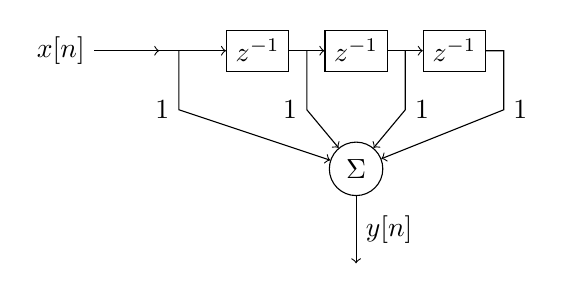
\begin{tikzpicture}[x=25mm,y=15mm]
	\node(x)at(0,0){$x[n]$};
	\node(z1)[draw,rectangle]at(1,0){$z^{-1}$};
	\node(z2)[draw,rectangle]at(1.5,0){$z^{-1}$};
	\node(z3)[draw,rectangle]at(2,0){$z^{-1}$};
	\node(s)[draw,circle]at(1.5,-1){$\Sigma$};
	\tikzset{every path/.style={->}}
	\draw(x)--(.5,0);
	\draw(.5,0)--(z1);
	\draw(z1)--(z2);
	\draw(z2)--(z3);
	\draw(.6,0)--+(0,-.5)node[left]{$1$}--(s);
	\draw(1.25,0)--+(0,-.5)node[left]{$1$}--(s);
	\draw(1.75,0)--+(0,-.5)node[right]{$1$}--(s);
	\draw(z3)--(2.25,0)--+(0,-.5)node[right]{$1$}--(s);
	\draw(s)--node[right]{$y[n]$}++(0,-.8);
\end{tikzpicture}
\end{document}
